\chapter{Introduction}
\label{chap:introduction}


% \section{Situation}
% \label{sec:situation}

People use financial services to save money, exchange currencies, borrow funds, make
payments, and earn interest. In traditional finance, these services are usually managed
by banks or other central organisations that approve transactions and maintain account
records. Decentralized Finance (DeFi) provides similar financial services through applications that operate on blockchain networks. A blockchain can be understood as a shared digital record that is maintained across multiple computers. Instead of relying on a central organisation to process financial operations, DeFi applications use smart contracts\footnote{A smart contract is executable code deployed at a blockchain address. Its functions process calls and update on-chain state according to the contract implementation and the current blockchain context.}. Smart contracts can implement operations such as token exchange, lending, borrowing, repayment, withdrawal, and asset transfer.

Users normally interact with DeFi applications through digital wallets. A wallet allows a user to control digital assets and approve blockchain transactions. In contrast to many traditional financial services, blockchain transactions are generally executed directly according to the information contained in the submitted transaction. Once confirmed, an incorrect transaction can be difficult or impossible to reverse. The broader ecosystem of blockchain-based applications is commonly referred to as Web3. Within this environment, users increasingly interact not only with conventional graphical interfaces but also with automated software systems. Recent developments in Large Language Models (LLMs) have enabled AI agents that can interpret natural-language instructions, select available tools, prepare structured parameters, and interact with external systems. Research on autonomous blockchain agents also describes increasing levels of automation, ranging from blockchain information retrieval to transaction preparation and delegated execution \cite{alqithamiAutonomousAgentsBlockchains2026}.

In this thesis, an AI agent is understood as a software component that interprets a user's natural-language request and converts it into structured information that can later be used for a blockchain operation. For example, a user could provide the instruction:

\begin{quote}
``Exchange 50 USDT for WETH using Uniswap\footnote{Uniswap is a decentralized exchange protocol that allows users to swap tokens through automated liquidity pools instead of a traditional order-book system. In this thesis, Uniswap is used as a representative example of a DeFi swap protocol.}.''
\end{quote}

USDT is a digital token designed to maintain a value close to the US dollar, while WETH, or Wrapped Ether, represents Ether in a token format that can be used by ERC-20-compatible applications.

An AI agent can make this interaction easier because the user does not need to know the exact smart-contract address, callable function, or other low-level blockchain details. The agent can translate the user's instruction into structured information and coordinate the technical components required to perform the action. Programmable smart accounts further support this type of automation. ERC-4337\footnote{ERC-4337 is an Ethereum standard that brings Account Abstraction to the network at the application layer without requiring core protocol changes. https://eips.ethereum.org/EIPS/eip-4337} allows smart accounts to apply programmable validation before an operation is executed. Research on ERC-4337 shows how this architecture separates account-specific validation from subsequent execution \cite{buterinERC4337AccountAbstraction2021,
linMeasurementInvestigationERC43372024}.

These developments create the possibility of a workflow in which a user describes a financial goal in ordinary language and an AI agent helps transform it into a blockchain action. At the same time, they introduce an important question: whether the transaction prepared by the automated system actually represents the financial action that the user intended.


% \section{Motivation}
% \label{sec:motivation}

% The ability to generate an executable action does not necessarily mean that the generated action is correct. This distinction becomes particularly important when AI systems are allowed to perform actions involving money or digital assets.

% Consider a small online business called \textit{BrightCart Studio}. The company regularly purchases packaging materials from an approved supplier. An employee gives an AI assistant the following instruction:

% \begin{quote}
% \textit{``Order 100 packaging boxes from our approved supplier.''}
% \end{quote}

% The instruction appears simple from the employee's perspective. However, the assistant must correctly identify the intended supplier, select the correct product, and use the appropriate payment destination. If the assistant selects the approved supplier and the correct payment information, the order can be completed as intended. However, the assistant could also select a website with a similar company name or an outdated supplier account. In such a case, the payment itself may still be technically valid: the bank account exists and the payment system can process the transaction. Nevertheless, the result does not correspond to what the employee requested.

% The payment system has not failed. It has correctly processed the information that it received. The problem occurred earlier because the AI-generated action was not checked against the user's intended business relationship.

% Figure~\ref{fig:motivation_scenario} illustrates this difference.

% \begin{figure}[htbp]
%     \centering
%     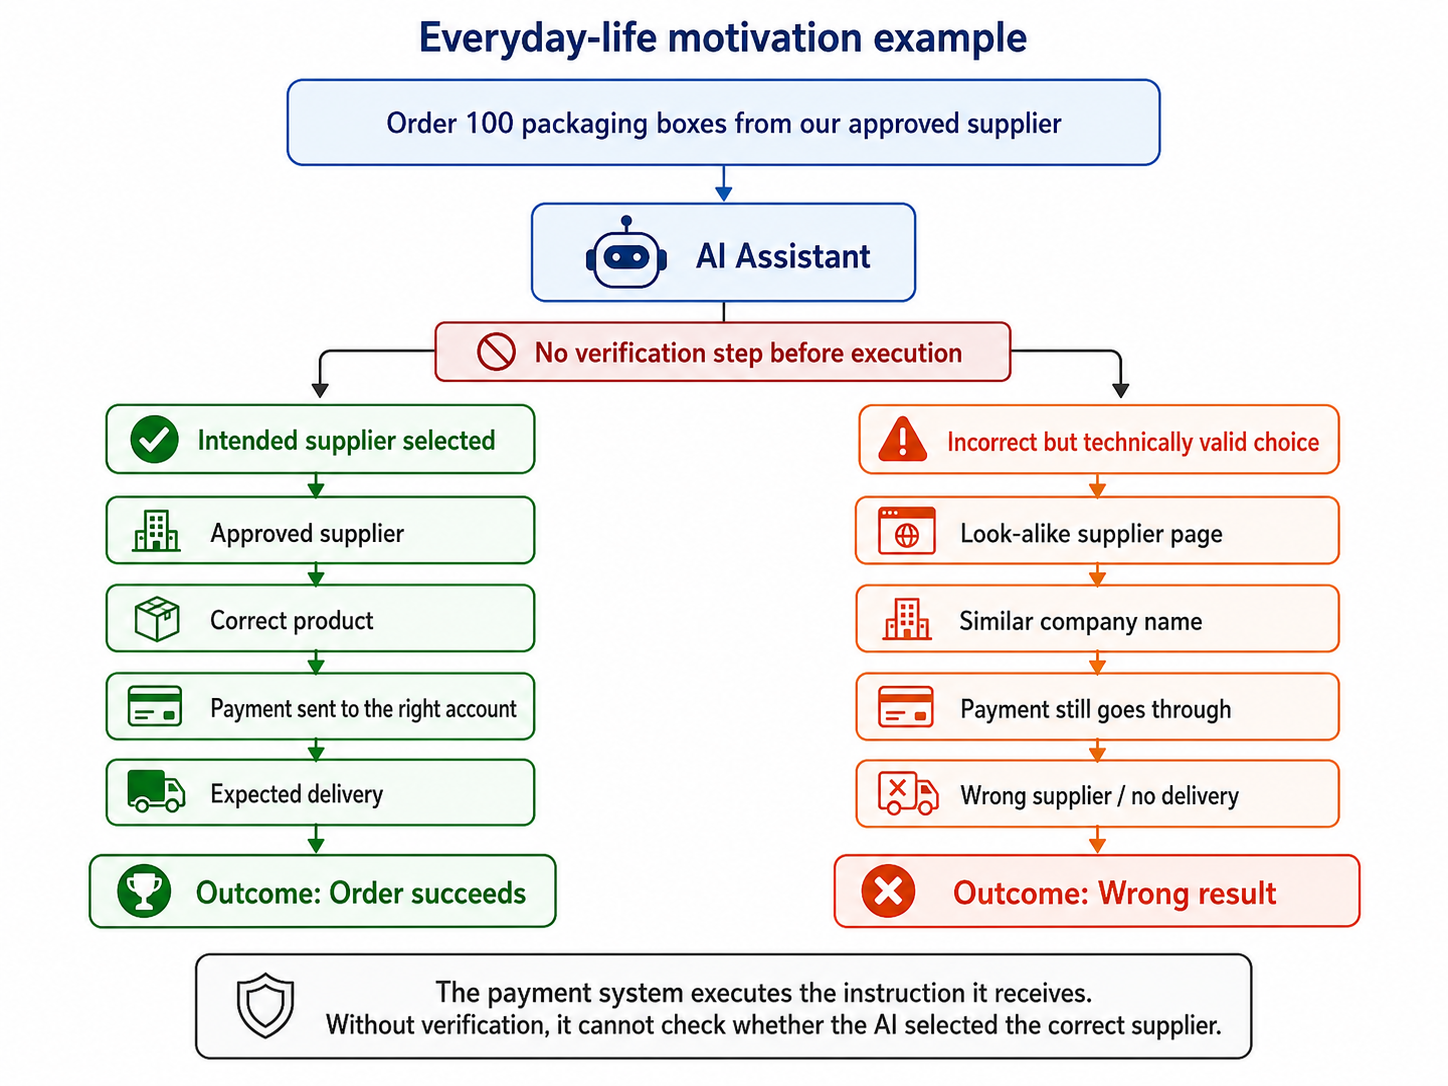
\includegraphics[width=0.88\textwidth]{figures/motivation_scenario.png}
%     \caption{An AI assistant may select either the intended supplier or an incorrect but technically valid supplier when no independent verification step is applied.(generated by GPT)}
%     \label{fig:motivation_scenario}
% \end{figure}

% The same situation can occur in DeFi. Consider the instruction:

% \begin{quote}
% \textit{``Supply 100 USDT to Aave\footnote{Aave is an Open Source Protocol to create Non-Custodial Liquidity Markets to earn interest on supplying and borrowing assets with a variable interest rate.} V3.''}
% \end{quote}

% The user expects a specific financial result: 100 USDT should be supplied to the intended Aave V3 market. To carry out this request, several technical elements must eventually correspond to each other. The operation must involve the correct protocol deployment, the requested action, an appropriate smart contract, a function capable of performing that action, and a supported USDT reserve.

% A transaction containing incorrect execution information may nevertheless be technically valid. It may be correctly encoded, digitally signed, accepted by a smart contract, and included in the blockchain. Technical execution therefore does not by itself establish that the transaction reflects the user's original request.

% This distinction is especially relevant in blockchain systems because confirmed transactions are difficult to reverse. A mistake involving the wrong contract, token, recipient, or function can therefore have direct financial consequences.

% The motivation for this thesis is not to replace existing wallet security, transaction simulation, digital signatures, or smart-contract security mechanisms. These mechanisms address important aspects of blockchain security. The motivation is to address a different question:

% \begin{quote}
% \textit{Does the transaction that is about to be constructed correspond to the DeFi action that the user actually requested?}
% \end{quote}

% Answering this question before execution would allow AI-assisted DeFi systems to combine the usability of natural-language interaction with an additional check of the intended execution relationship.

\section{Motivation}
\label{sec:motivation}

An AI assistant can prepare an instruction that a payment system accepts
even when the funds are directed to the wrong destination. Consider
\textit{BrightCart Studio}, a small online business whose employee asks
an assistant to ``order 100 packaging boxes from our approved supplier.'' BrightCart's supplier record identifies Account A as the registered
payment account for Supplier A. As Figure~\ref{fig:motivation_scenario}
shows, the assistant selects Supplier A but enters Account B in the
payment instruction. If Account B can receive the payment and the
instruction passes the payment system's checks, the payment may be
processed. The error lies in the association between the supplier and
the account selected for payment.

\begin{figure}[H]
    \centering
    % \begingroup
% \definecolor{motfill}{HTML}{F8FAFC}
% \definecolor{motborder}{HTML}{475569}
% \definecolor{motarrow}{HTML}{64748B}
% \definecolor{mottext}{HTML}{1E293B}
% \definecolor{motaccent}{HTML}{9A4A32}
% \begin{tikzpicture}[
%     >=stealth,
%     font=\sffamily\fontsize{10}{12}\selectfont,
%     box/.style={draw=motborder, fill=motfill, text=mottext,
%         line width=0.6pt, rounded corners=2pt,
%         align=center, inner xsep=8pt, inner ysep=9pt},
%     panel/.style={box, text width=5.4cm, minimum height=2.9cm},
%     flow/.style={->, draw=motarrow, line width=0.85pt,
%         shorten <=2pt, shorten >=2pt},
%     compare/.style={->, draw=motarrow, line width=0.85pt,
%         shorten <=2pt, shorten >=2pt},
%     icon/.style={draw=motborder, line width=0.8pt,
%         line cap=round, line join=round},
%     pics/person/.style={code={
%         \draw[icon] (0,0.12) circle (0.11);
%         \draw[icon] (-0.22,-0.22) .. controls (-0.22,0.02)
%             and (0.22,0.02) .. (0.22,-0.22) -- cycle;
%     }},
%     pics/record/.style={code={
%         \draw[icon] (-0.18,-0.23) rectangle (0.18,0.23);
%         \foreach \y in {-0.12,0,0.12}
%             \draw[icon] (-0.10,\y) -- (0.10,\y);
%     }},
%     pics/ai/.style={code={
%         \draw[icon,rounded corners=1pt]
%             (-0.18,-0.18) rectangle (0.18,0.18);
%         \foreach \p in {-0.09,0.09}{
%             \draw[icon] (\p,0.18) -- (\p,0.27);
%             \draw[icon] (\p,-0.18) -- (\p,-0.27);
%             \draw[icon] (0.18,\p) -- (0.27,\p);
%             \draw[icon] (-0.18,\p) -- (-0.27,\p);
%         }
%         \node[text=motborder,font=\sffamily\tiny] at (0,0) {AI};
%     }},
%     pics/mismatch/.style={code={
%         \draw[icon,draw=motaccent] (0,0) circle (0.23);
%         \draw[icon,draw=motaccent] (-0.11,0.06) -- (0.11,0.06);
%         \draw[icon,draw=motaccent] (-0.11,-0.06) -- (0.11,-0.06);
%         \draw[icon,draw=motaccent] (-0.07,-0.15) -- (0.07,0.15);
%     }},
%     pics/payment/.style={code={
%         \draw[icon,rounded corners=1pt]
%             (-0.28,-0.18) rectangle (0.28,0.18);
%         \draw[icon] (-0.28,0.05) -- (0.28,0.05);
%         \draw[icon] (-0.19,-0.09) -- (-0.04,-0.09);
%     }}
% ]
% \node[box, text width=11.9cm] (request) at (0,0)
%     {\rule{0pt}{0.48cm}\\[2pt]\textbf{Employee request}\\[4pt]
%     ``Order 100 packaging boxes from our approved supplier.''};

% \node[panel] (record) at (-3.25,-3.25)
%     {\rule{0pt}{0.48cm}\\[2pt]\textbf{Approved supplier record}\\[7pt]
%     Supplier A\\[4pt]
%     Registered account: \textbf{Account A}};

% \node[panel] (candidate) at (3.25,-3.25)
%     {\rule{0pt}{0.48cm}\\[2pt]\textbf{AI payment instruction}\\[7pt]
%     Supplier A\\[4pt]
%     Selected account: \textcolor{motaccent}{\textbf{Account B}}};

% \pic at ([yshift=-0.40cm]request.north) {person};
% \pic at ([yshift=-0.45cm]record.north) {record};
% \pic at ([yshift=-0.45cm]candidate.north) {ai};

% \draw[flow] (request.south -| record.north) -- (record.north);
% \draw[flow] (request.south -| candidate.north) -- (candidate.north);

% \node[box, draw=motaccent, text width=11.9cm] (mismatch) at (0,-6.2)
%     {\rule{0pt}{0.48cm}\\[2pt]\textbf{Account mismatch}};

% \pic at ([yshift=-0.40cm]mismatch.north) {mismatch};

% \draw[compare] (record.south) -- (record.south |- mismatch.north);
% \draw[compare] (candidate.south) -- (candidate.south |- mismatch.north);

% \node[box, text width=11.9cm] (consequence) at (0,-8.75)
%     {\rule{0pt}{0.48cm}\\[2pt]\textbf{Without verification}\\[4pt]
%     Payment may reach the wrong account.};
% \pic at ([yshift=-0.40cm]consequence.north) {payment};
% \draw[flow] (mismatch.south) -- (consequence.north);
% \end{tikzpicture}
% \endgroup

% Requires \usepackage{tikz}. Drawing only; keep the figure
% environment and its label in the introduction chapter.
\begingroup
\definecolor{motborder}{HTML}{475569}
\definecolor{motfill}{HTML}{F8FAFC}
\definecolor{mottext}{HTML}{1E293B}
\definecolor{motaccent}{HTML}{914832}

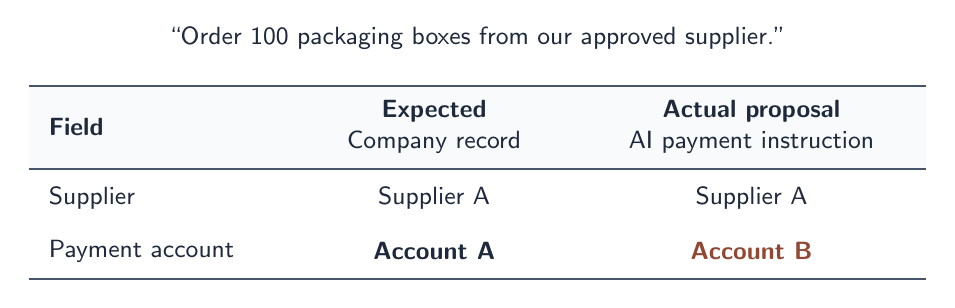
\begin{tikzpicture}[
    x=1cm, y=1cm,
    font=\sffamily\small,
    every node/.style={text=mottext, inner sep=0pt}
]
% The request provides context for both columns.
\node[align=center, text width=11.4cm] at (0,0)
    {``Order 100 packaging boxes from our approved supplier.''};

% Comparison table: fields at left, expected and proposed values at right.
\fill[motfill] (-5.7,-0.60) rectangle (5.7,-1.65);
\draw[motborder, line width=0.7pt]
    (-5.7,-0.60) -- (5.7,-0.60)
    (-5.7,-1.65) -- (5.7,-1.65)
    (-5.7,-3.05) -- (5.7,-3.05);

\node[anchor=west, font=\sffamily\small\bfseries]
    at (-5.45,-1.12) {Field};
\node[align=center] at (-0.55,-1.12)
    {\textbf{Expected}\\Company record};
\node[align=center] at (3.48,-1.12)
    {\textbf{Actual proposal}\\AI payment instruction};

\node[anchor=west] at (-5.45,-2.03) {Supplier};
\node at (-0.55,-2.03) {Supplier A};
\node at (3.48,-2.03) {Supplier A};

\node[anchor=west] at (-5.45,-2.70) {Payment account};
\node at (-0.55,-2.70) {\textbf{Account A}};
\node[text=motaccent] at (3.48,-2.70) {\textbf{Account B}};
\end{tikzpicture}
\endgroup
    \caption{BrightCart's registered payment details and the assistant's
    proposal.}
    \label{fig:motivation_scenario}
\end{figure}

In DeFi, the corresponding question is whether the selected contract
belongs to the intended market. Consider the request:

\begin{quote}
\textit{``Supply 100 USDT to Aave V3.''}\footnote{Aave is a
decentralised liquidity protocol that supports supplying and borrowing
cryptoassets. For an empirical study of lending markets including Aave,
see Gudgeon et al.~\cite{gudgeonLoanableFunds2020}. For the Aave V3 Pool
contract, see \url{https://aave.com/docs/aave-v3/smart-contracts/pool}.}
\end{quote}

The request specifies the action, asset, and amount, but leaves the
network and market unstated. Suppose the execution context identifies
the network and Market A as the intended Aave V3 market. The supply
operation then requires the Pool contract for Market A, its supply
function, and the USDT reserve supported by that market.

In Figure~\ref{fig:aave_supply_comparison}, the assistant preserves
the instruction to supply 100 USDT but selects Pool B, which belongs
to Market B on the same network. If Market B supports the same token
and the call meets its execution conditions, the transaction could
succeed. The funds would then be supplied to Market B even though
Market A was intended.

\begin{figure}[htbp]
    \centering
    % Drawing only. Requires \usepackage{tikz}.
\begingroup
\definecolor{motInk}{HTML}{1E293B}
\definecolor{motRule}{HTML}{475569}
\definecolor{motLight}{HTML}{F1F5F9}
\definecolor{motRust}{HTML}{853E2D}
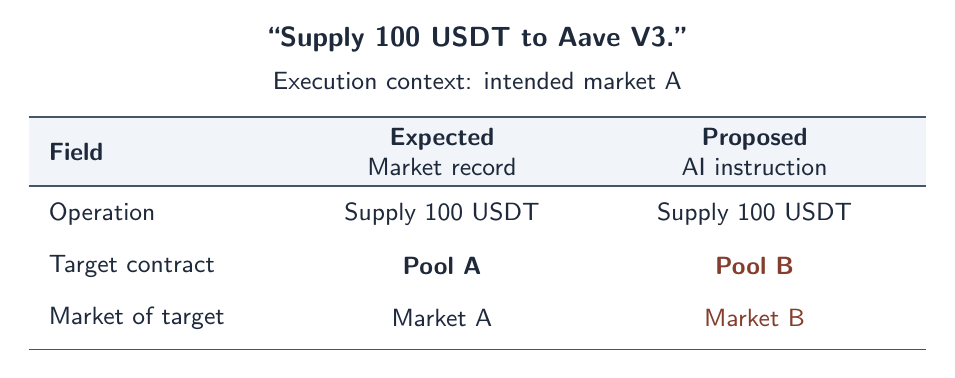
\begin{tikzpicture}[x=1cm,y=1cm,font=\sffamily\small,
every node/.style={text=motInk,inner sep=0pt}]
\node[align=center,font=\sffamily\bfseries] at (0,0)
  {\textquotedblleft Supply 100 USDT to Aave V3.\textquotedblright};
\node[align=center,font=\sffamily\small] at (0,-.52)
  {Execution context: intended market A};
\fill[motLight] (-5.7,-.98) rectangle (5.7,-1.85);
\draw[motRule,line width=.65pt] (-5.7,-.98)--(5.7,-.98)
 (-5.7,-1.85)--(5.7,-1.85) (-5.7,-3.93)--(5.7,-3.93);
\node[anchor=west,font=\sffamily\small\bfseries] at (-5.45,-1.42) {Field};
\node[align=center] at (-.45,-1.42) {\textbf{Expected}\\Market record};
\node[align=center] at (3.52,-1.42) {\textbf{Proposed}\\AI instruction};
\node[anchor=west] at (-5.45,-2.21) {Operation};
\node at (-.45,-2.21) {Supply 100 USDT};
\node at (3.52,-2.21) {Supply 100 USDT};
\node[anchor=west] at (-5.45,-2.87) {Target contract};
\node at (-.45,-2.87) {\textbf{Pool A}};
\node[text=motRust] at (3.52,-2.87) {\textbf{Pool B}};
\node[anchor=west] at (-5.45,-3.53) {Market of target};
\node at (-.45,-3.53) {Market A};
\node[text=motRust] at (3.52,-3.53) {Market B};
\end{tikzpicture}
\endgroup
    \caption{Expected and proposed Pool contracts for the same Aave V3
    supply request.}
    \label{fig:aave_supply_comparison}
\end{figure}

Related work illustrates why the identity behind an address matters.
Tsuchiya et al.\ document transfers to unintended addresses that
resembled those of familiar recipients
\cite{tsuchiyaAddressPoisoning2025}. Gallersd\"orfer et al.\ examine
how a wallet can verify the association between a website and a
contract address \cite{gallersdorferMetaMaskTLS2022}. The Aave example
requires a distinct check: even a legitimate Pool contract can be
inappropriate for a request if it belongs to a different market.

This thesis complements wallet controls, transaction simulation,
digital signatures, and smart-contract security analysis by asking
the following question before transaction construction:

\begin{quote}
\textit{Does authoritative information for the selected network and
market support the execution relationships required by the proposed
DeFi operation?}
\end{quote}

Approval means that the mandatory relationships for the structured
operation have been established within the supported scope. It does
not establish that the assistant interpreted the original request
correctly, guarantee successful execution, or predict a favourable
financial outcome. If the evidence is incomplete or outdated to the
extent that a required relationship cannot be established, the
operation must not be approved.

% \section{Problem Analysis}
% \label{sec:problem_analysis}

% The motivating example represents one instance of a broader problem. AI-driven DeFi workflows contain several stages at which incomplete, incorrect, or mismatched information can influence the final transaction. Research on autonomous blockchain agents identifies related risks involving intent formulation, delegated execution, authorization, policy misuse, and transaction pipelines \cite{alqithamiAutonomousAgentsBlockchains2026}.

% The main sub-problems relevant to this thesis are described below.


% \subsection{Natural-Language Requests Can Be Incomplete or Ambiguous}
% \label{subsec:natural_language_problem}

% Users normally describe financial actions in ordinary language rather than through complete blockchain transaction parameters.

% For example:

% \begin{quote}
% ``Swap WETH for USDT.''
% \end{quote}

% This request does not specify an amount, blockchain network, protocol deployment, or other action-specific information.

% Similarly:

% \begin{quote}
% ``Supply USDT to Aave.''
% \end{quote}

% does not specify the amount, network, Aave market, or exact asset representation.

% An AI agent may attempt to infer missing information. However, an automatically inferred value may differ from what the user intended. A secure workflow must therefore distinguish information that describes the user's financial intention from technical information that can be resolved later. Critical ambiguity must not silently become part of an executable financial operation.


% \subsection{AI-Generated Information Can Be Plausible but Incorrect}
% \label{subsec:probabilistic_ai_problem}

% LLMs are useful for interpreting natural language, but their outputs are probabilistic. A generated result may appear clear and technically convincing while still containing incorrect or mismatched information. Retrieval-Augmented Generation can improve access to external and more current information, but retrieval does not automatically guarantee that the retrieved information is authoritative, complete, or correctly interpreted. The final result may still contain an incorrect protocol, action, asset, address, or function.

% This creates a security problem when the same generated information is used directly to construct a financial transaction. The correctness of an AI-generated action should therefore not depend only on the confidence or plausibility of the language-model output.


% \subsection{DeFi Actions Require Different Execution Relationships}
% \label{subsec:action_specific_problem}

% Different DeFi operations require different \textbf{execution relationships}. 
% For example, a \textit{token swap} typically connects an input asset and an output asset with an exchange protocol, router contract, swap function, and supported liquidity pool or token pair. 
% A \textit{lending operation}, in contrast, connects a lending protocol with a supported reserve asset, protocol contract, action-specific function, and amount. 
% Therefore, the required verification depends on the \textbf{type of DeFi action} being performed. Transfers and token approvals require different information again.

% Therefore, verifying only one isolated value is insufficient. For example, confirming that a contract belongs to Aave does not prove that it is the correct contract for the requested action. Likewise, confirming that USDT is a known token does not prove that it is supported by the selected protocol deployment.

% The relevant entities must form the correct action-specific execution relationship.


% \subsection{Human-Readable Names Are Not Sufficient Identifiers}
% \label{subsec:identifier_problem}

% Users naturally refer to protocols and assets using names such as ``Aave'', ``Uniswap'', ``USDT'', or ``WETH''. Blockchain execution, however, ultimately depends on network-specific contract addresses, functions, and encoded parameters. A token symbol may exist on several blockchain networks, and different contracts may use identical or similar names. A contract may also use terminology associated with a well-known protocol without belonging to an official deployment.

% Consequently, a correct interpretation at the language level does not automatically provide an authoritative blockchain identifier. The relationship between human-readable intent and the corresponding on-chain entities must be established before execution.


% \subsection{Authorization and Intent Correctness Are Different Problems}
% \label{subsec:authorization_problem}

% Programmable wallets can restrict the actions available to an automated agent. For example, a wallet may limit the maximum amount that can be spent or restrict transactions to selected contracts. ERC-4337 and related programmable-account mechanisms provide an important basis for such controlled execution \cite{buterinERC4337AccountAbstraction2021,
% linMeasurementInvestigationERC43372024}.

% These mechanisms primarily answer an authorization question:

% \begin{quote}
% ``Is this agent permitted to execute this operation?''
% \end{quote}

% However, authorization does not necessarily answer:

% \begin{quote}
% ``Is this operation the correct interpretation of the user's request?''
% \end{quote}

% For example, an agent may have permission to interact with both Uniswap and Aave. If it prepares a Uniswap swap when the user requested an Aave supply action, the operation could remain within the wallet's permissions while still being inconsistent with the user's intention.

% Authorization and intent correctness must therefore be treated as separate concerns.


% \subsection{Verification Depends on Current and Authoritative Information}
% \label{subsec:trusted_information_problem}

% The correctness of a DeFi execution path depends on information about protocol deployments, smart contracts, callable functions, pools, reserves, assets, and blockchain networks. This information may change. Protocols can introduce new deployments, add supported assets, update integrations, or deprecate earlier components. Information that was once correct may therefore become outdated.

% A verification mechanism that uses outdated or untrusted information can produce incorrect decisions even when its internal checking process behaves consistently. The source and freshness of verification information are therefore part of the problem itself.


% \subsection{Problem Statement}
% \label{subsec:problem_statement}

% The preceding sub-problems lead to the central problem addressed by this thesis:

% \begin{quote}
% \textbf{The problem addressed in this thesis is how to verify, before blockchain execution, that an AI-generated DeFi transaction intent is consistently mapped to the intended protocol deployment, action, authoritative smart contract, callable function, and supported asset or protocol resource.}
% \end{quote}

% Figure~\ref{fig:problem_statement_overview} summarises the position of this problem within an AI-driven DeFi workflow.

% \begin{figure}[htbp]
%     \centering
%     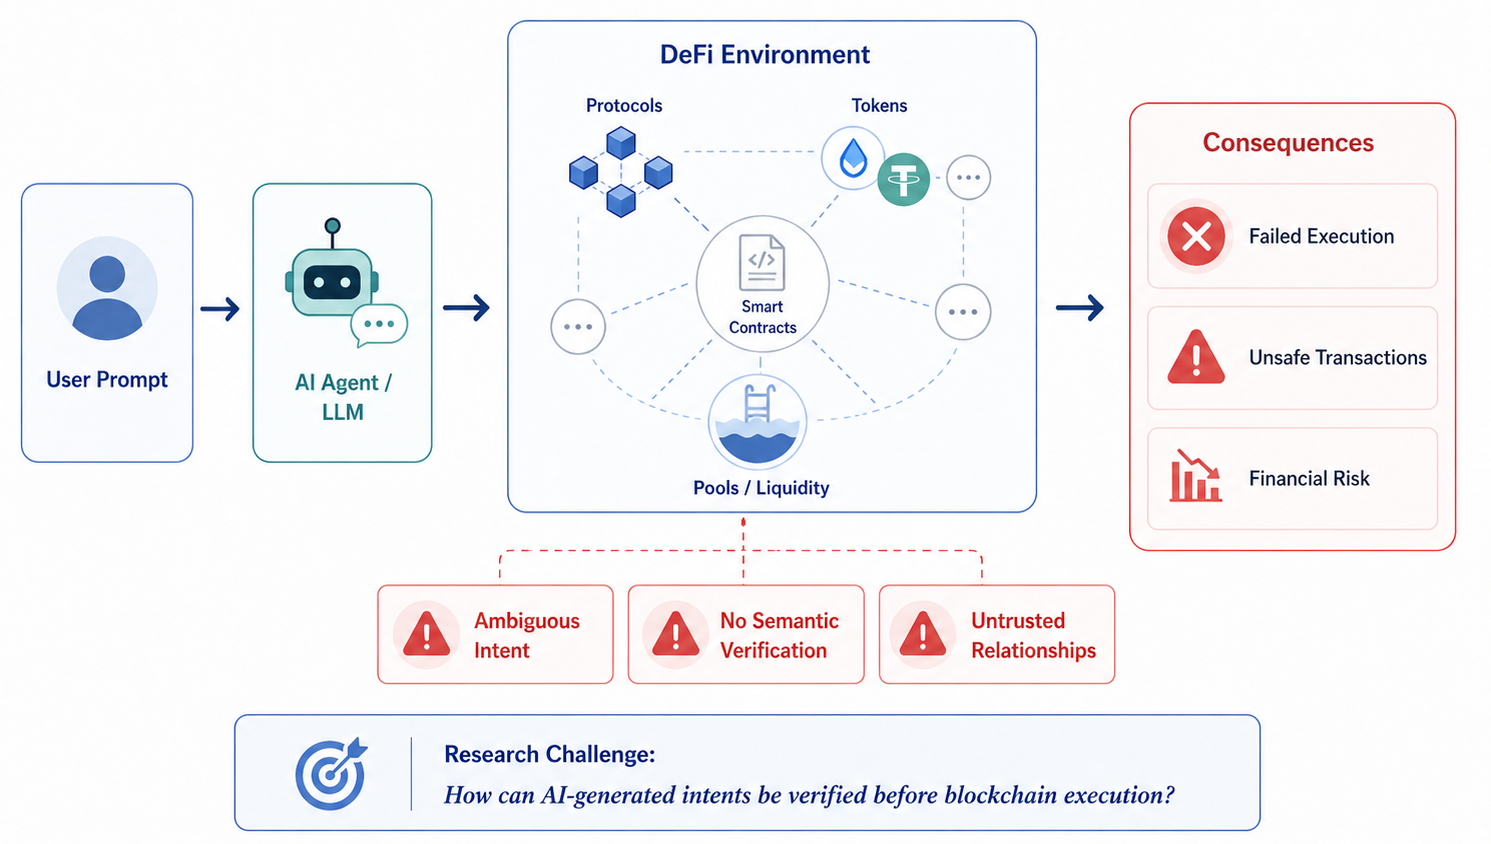
\includegraphics[width=0.90\textwidth]{figures/problem_statement_overview.png}
%     \caption{The verification problem investigated between AI-generated DeFi intent and blockchain transaction construction.(generated by GPT)}
%     \label{fig:problem_statement_overview}
% \end{figure}

% The problem is located after the user's request has been interpreted but before the corresponding blockchain transaction is constructed and executed. The required check concerns not only individual entities, but also whether those entities form the correct relationship for the requested financial action.
\section{Problem Analysis}
\label{sec:problem_analysis}

% Bold, unnumbered headings on their own line; keep each with its paragraph.
\providecommand{\problemheading}[1]{%
  \par\addvspace{0.8\baselineskip}%
  \noindent\textbf{#1}\par\nobreak\smallskip\nobreak
  \noindent\ignorespaces}

The supply example illustrates how an assistant can preserve the requested
action and amount yet select a contract belonging to the wrong market.
Research on autonomous blockchain agents identifies related risks in intent
formulation, delegated execution, authorisation, and transaction preparation
\cite{alqithamiAutonomousAgentsBlockchains2026}. The first three subproblems concern incomplete or ambiguous requests,
plausible but incorrect model outputs, and execution relationships that
cannot be verified by checking entities in isolation. The remaining three
concern the difficulty of resolving names to on-chain identifiers, the
limits of wallet authorisation as evidence of user intent, and the
reliability of the information used for verification.

\problemheading{Incomplete or ambiguous requests}
A request can be incomplete even when the intended action is clear.
Consider the instruction:

\begin{quote}
\textit{``Swap WETH for USDT.''}
\end{quote}

The user has specified the swap direction but has not said how much WETH
to exchange. Identifying the appropriate deployment or pool cannot resolve
that omission. By contrast, consider a request that specifies the amount:

\begin{quote}
\textit{``I need 100 USDT from Aave.''}
\end{quote}

Here the uncertainty concerns the action. Depending on the user's position,
the request could mean withdrawing previously supplied USDT or borrowing
USDT. Both could put the same amount in the user's wallet, but withdrawing
reduces a supplied balance, whereas borrowing creates a debt. If the
context does not distinguish these intentions, the assistant must seek
clarification or stop before preparing the operation. Technical details present a different case. Once the action and execution
context are established, contract addresses can be resolved from
authoritative information. An explicit application policy may also supply
a default network when the user omits it, but must not override a network
the user specifies.

\problemheading{Plausible but incorrect AI interpretations}
LLMs are useful for interpreting natural language, but their outputs
are probabilistic. A generated result may appear clear and technically
convincing while containing incorrect or mismatched information.
Retrieval-Augmented Generation can improve access to external
information, including information that is more recent than the model's
training data. However, retrieval does not automatically establish that
the information is authoritative, complete, current, or correctly
interpreted. The generated result may still contain an incorrect
protocol, action, asset, address, or function.

This creates a security problem when generated information is used
directly to construct a financial transaction. A plausible explanation
or a structurally valid output does not establish that the proposed
operation is supported by the selected protocol deployment. The
correctness of an AI-generated action should therefore not depend
solely on the apparent confidence or plausibility of the model's output. Two forms of correctness must be distinguished. The first concerns
whether the structured intent accurately represents the user's request.
The second concerns whether the execution relationships required by
that intent can be established from authoritative information. An
incorrectly interpreted request may still describe an operation with
valid execution relationships. Interpretation correctness and
relationship verification must therefore be assessed separately.


\problemheading{Valid entities with incompatible execution relationships}
For a token swap, the selected contract and function must support the
exchange, and the chosen pool or route must connect the input and output
assets. For a lending operation, the contract must belong to the selected
market, the function must perform the requested action, and the asset must
correspond to a supported reserve. A function that borrows an asset cannot
serve a request to repay it, even if both functions belong to the same
contract. Checking each entity independently misses this distinction. A Pool contract
may belong to Aave V3 and a token contract may identify USDT on the
selected network, yet the Pool may belong to another market or may not
support that reserve. Verification must therefore establish the
relationships required by the particular action and deployment.

\problemheading{Ambiguous protocol and asset identifiers}
Users naturally refer to protocols and assets using names such as
``Aave'', ``Uniswap'', ``USDT'', or ``WETH''. Blockchain execution,
however, depends on network-specific contract addresses, functions,
and encoded parameters. A token symbol may be used on several
blockchain networks, and different contracts may use identical or
similar names. A contract may also use terminology associated with a
well-known protocol without belonging to an official deployment. Consequently, a correct interpretation of a name at the language level
does not provide an authoritative blockchain identifier. Resolving
``USDT'', for example, requires identifying the relevant token contract
within the applicable network and establishing its relationship to
the selected protocol resource.

The mapping from human-readable intent to on-chain entities must
therefore be grounded in authoritative information. A matching name
alone is insufficient evidence that a contract, asset, or protocol
resource is appropriate for the requested operation.


\problemheading{Wallet permissions do not establish user intent}
Programmable wallets can restrict the actions available to an automated
agent. Depending on their implementation, wallet policies may limit
spending amounts or restrict interactions to selected contracts.
ERC-4337 and related programmable-account mechanisms provide a basis
for implementing such controlled execution
\cite{buterinERC4337AccountAbstraction2021,
linMeasurementInvestigationERC43372024}.

These controls address an authorisation question:

\begin{quote}
\textit{``Is this agent permitted to execute this operation?''}
\end{quote}

Authorisation does not necessarily answer:

\begin{quote}
\textit{``Does this operation correspond to the user's request?''}
\end{quote}

For example, an agent may have permission to interact with both Uniswap
and Aave. If it prepares a Uniswap swap when the user requested an Aave
supply action, the operation could remain within the wallet's
permissions while being inconsistent with the user's intention. This example also illustrates the boundary of relationship
verification. If the incorrectly generated swap intent describes a
supported Uniswap operation, its execution relationships may be valid.
Checking those relationships alone would not reveal that the user
originally requested a different action.

Interpretation correctness, relationship verification, and execution
authorisation must therefore be treated as separate concerns. Within
this distinction, the central verification task of this thesis is to
establish whether the structured DeFi intent is consistent with the
authoritative execution relationships required for the proposed
operation.


\problemheading{Outdated or incomplete verification evidence}
The correctness of a DeFi execution structure depends on information
about protocol deployments, smart contracts, callable functions, pools,
reserves, assets, and blockchain networks. This information may change.
Protocols can introduce new deployments, add supported assets, update
integrations, or deprecate earlier components. Information that was
once correct may therefore become outdated. A verification mechanism that relies on outdated or untrusted
information can produce incorrect decisions even when its internal
checking process behaves consistently. The source and freshness of
verification knowledge are therefore part of the problem itself. Completeness is also relevant. If a required relationship is absent
from the available knowledge, this absence does not necessarily
establish that the operation is unsupported. It may instead indicate
incomplete coverage or a failed acquisition or update process.
Treating an absent relationship as evidence of an unsupported operation
requires sufficiently complete and current knowledge for the relevant
verification scope.

The verification process must therefore distinguish evidence of an
unsupported or inconsistent operation from insufficient evidence to
reach a decision. When the required relationships cannot be established
reliably, the operation must not be approved.


\problemheading{Problem statement}
These subproblems lead to the central question of this thesis:

\begin{quote}
\textbf{Before a transaction is constructed, how can a verifier establish
whether authoritative information supports the relationships that an
AI-generated structured DeFi intent requires among the network, protocol
deployment, action, contract, function, and relevant assets, pools, or
reserves?}
\end{quote}

Figure~\ref{fig:problem_statement_overview} shows where a mismatch can
pass unnoticed if a structured intent is used directly for transaction
construction. The solid arrows show the processing sequence. The
annotation marks the transition at which evidence for the proposed
relationships is needed. If a mismatch goes unchecked, the transaction
may fail, or it may execute against an unintended target.

\begin{figure}[H]
    \centering
    \begingroup
\definecolor{probfill}{HTML}{F8FAFC}
\definecolor{probborder}{HTML}{475569}
\definecolor{probtext}{HTML}{1E293B}
\definecolor{probaccent}{HTML}{984A35}
\definecolor{probgap}{HTML}{FCF8F6}
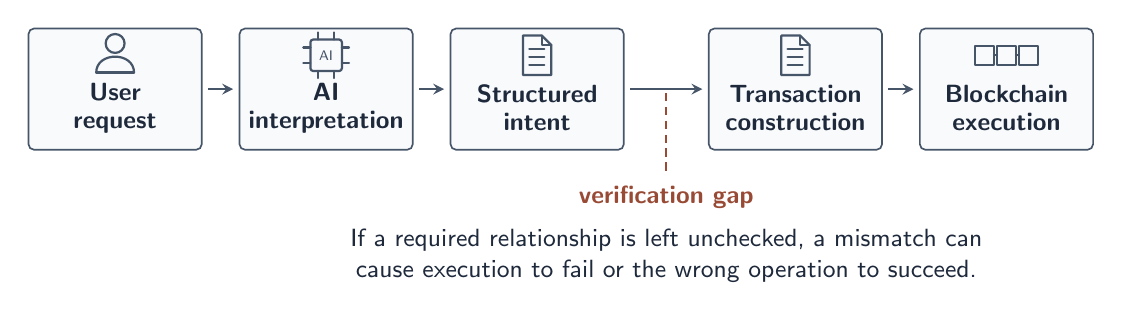
\begin{tikzpicture}[
    >=stealth,
    font=\sffamily\fontsize{10}{12}\selectfont,
    box/.style={draw=probborder,fill=probfill,text=probtext,
      rounded corners=2pt,line width=0.6pt,align=center,
      inner xsep=7pt,inner ysep=8pt},
    flow/.style={->,draw=probborder,line width=0.75pt,
      shorten <=2pt,shorten >=2pt},
    icon/.style={draw=probborder,line width=0.8pt,line cap=round,
      line join=round},
    pics/person/.style={code={
      \draw[icon] (0,0.15) circle (0.12);
      \draw[icon] (-0.24,-0.22) .. controls (-0.24,0.05)
        and (0.24,0.05) .. (0.24,-0.22);
      \draw[icon] (-0.24,-0.22)--(0.24,-0.22);
    }},
    pics/chip/.style={code={
      \draw[icon,rounded corners=1pt] (-0.2,-0.2) rectangle (0.2,0.2);
      \foreach \p in {-0.1,0.1}{
        \draw[icon] (\p,0.2)--(\p,0.29);
        \draw[icon] (\p,-0.2)--(\p,-0.29);
        \draw[icon] (0.2,\p)--(0.29,\p);
        \draw[icon] (-0.2,\p)--(-0.29,\p);
      }
      \node[text=probborder,font=\sffamily\tiny] at (0,0) {AI};
    }},
    pics/document/.style={code={
      \draw[icon] (-0.18,-0.25)--(0.18,-0.25)--(0.18,0.13)
        --(0.06,0.25)--(-0.18,0.25)--cycle;
      \draw[icon] (0.06,0.25)--(0.06,0.13)--(0.18,0.13);
      \foreach \p in {-0.12,-0.02,0.08}
        \draw[icon] (-0.10,\p)--(0.09,\p);
    }},
    pics/blocks/.style={code={
      \draw[icon] (-0.4,-0.12) rectangle (-0.16,0.12);
      \draw[icon] (-0.12,-0.12) rectangle (0.12,0.12);
      \draw[icon] (0.16,-0.12) rectangle (0.4,0.12);
      \draw[icon] (-0.16,0)--(-0.12,0);
      \draw[icon] (0.12,0)--(0.16,0);
    }}
]
% Only the five stages use boxes and arrows. The note is a margin annotation.
\foreach \id/\x/\glyph/\title in {
    req/0/person/{User\\request},interp/2.68/chip/{AI\\interpretation},
    cand/5.36/document/{Structured\\intent},build/8.64/document/{Transaction\\construction},
    exec/11.32/blocks/{Blockchain\\execution}}{
    \node[box,minimum width=2.20cm,minimum height=1.54cm] (\id) at (\x,0) {};
    \pic at (\x,0.43) {\glyph};
    \node[align=center,text=probtext,font=\sffamily\bfseries\fontsize{9}{10.2}\selectfont]
        at (\x,-0.24) {\title};
}
\draw[flow] (req.east)--(interp.west);
\draw[flow] (interp.east)--(cand.west);
\draw[flow] (cand.east)--(build.west);
\draw[flow] (build.east)--(exec.west);

% Non-directional leader touches the transition, not either stage.
\draw[draw=probaccent,densely dashed,line width=0.65pt]
    (7.00,-0.05)--(7.00,-1.08);
\node[anchor=north,text=probaccent,font=\sffamily\bfseries\small]
    at (7.00,-1.11) {verification gap};
\node[anchor=north,align=center,text=probtext,font=\sffamily\small]
    at (7.00,-1.66) {If a required relationship is left unchecked, a mismatch can\\
                      cause execution to fail or the wrong operation to succeed.};
\end{tikzpicture}
\endgroup
    \caption[Verification gap before transaction construction]{Verification gap before transaction construction in DeFi.}
    \label{fig:problem_statement_overview}
\end{figure}

The proposed verifier addresses this gap by checking the structured intent
against authoritative knowledge. Approval requires evidence for every
mandatory relationship within the supported scope. An established
mismatch and insufficient evidence both prevent the operation from
proceeding, although they are distinct findings. Only an approved
structured verification result may be used to construct the transaction;
the execution component must not reconstruct the operation from the
original request. Approval neither establishes that the model interpreted
the request correctly nor guarantees successful execution or a favourable
financial outcome.


\section{Objectives and Scope}
\label{sec:objectives_scope}

The main objective of this thesis is to investigate whether an
automatically populated, domain-specific property graph can verify the
execution relationships required by an AI-generated DeFi intent before
transaction construction, and how the resulting decision can be used
in a controlled ERC-4337 wallet workflow.

Research on knowledge graphs and large language models examines how
explicit relationships can support the use of external knowledge
\cite{panUnifyingLargeLanguage2024}. Graph-based retrieval approaches
also use these relationships to retrieve information across connected
entities \cite{hanRetrievalAugmentedGenerationGraphs2025,
hanRAGVsGraphRAG2026}. In this thesis, the graph serves a different
purpose: it provides the evidence against which a proposed operation
is checked.

The six sub-objectives below correspond, in order, to the six
sub-problems identified in Section~\ref{sec:problem_analysis}:

\begin{enumerate}
    \item \textbf{Identify missing or ambiguous intent information.}
    Translate selected natural-language requests into machine-readable
    intents and distinguish information established by the request or
    the configured execution context from information that still
    requires clarification.

    \item \textbf{Check AI-generated proposals against independent
    evidence.}
    Assess the operation proposed by the assistant against protocol
    and blockchain information obtained independently of the language
    model. A plausible interpretation is not sufficient grounds for
    approval.

    \item \textbf{Verify the relationships required by each action.}
    Represent and check how the deployment, contract, function, and
    assets must be connected for the proposed action, including the
    relevant pool or reserve where applicable. The presence of each
    entity in the graph is insufficient if the required connections
    do not hold.

    \item \textbf{Resolve names to identifiers on the selected network.}
    Establish which deployment, contract, and token identifiers
    correspond to the protocol and asset names used in a structured
    intent. This allows the verifier to distinguish entities that
    share a name or symbol.

    \item \textbf{Distinguish intent verification from wallet
    authorisation.}
    Investigate how a controlled ERC-4337 wallet workflow can use the
    verification result so that only an approved operation proceeds
    to transaction construction. Permission to call a contract does
    not, by itself, establish that the contract is appropriate for
    the requested action.

    \item \textbf{Account for the source, freshness, and completeness
    of verification evidence.}
    Automatically populate the graph from configured authoritative
    sources and distinguish evidence of a mismatch from a case in
    which the available information is too incomplete or outdated
    to support a decision.
\end{enumerate}

The evaluation assesses these objectives across supported and
unsupported operations. It examines verification effectiveness,
repeatability, decision traceability, processing time, and the extent
to which the graph can be extended without redesigning the
verification model.

\medskip
\noindent\textbf{Scope.}
The prototype is evaluated on Ethereum Sepolia and covers two protocols
with different execution relationships. For Uniswap V3, it considers
single-hop token swaps, for which the selected router and swap function
must support the operation and the pool must correspond to the
requested token pair. For Aave V3, it considers supply, withdrawal,
borrowing, and repayment, for which the selected Pool contract,
function, and reserve asset must correspond to the intended market
and action. The asset scope includes USDT and WETH. Protocol-specific ingestion components populate the graph with the
entities and relationships needed for these operations. The bounded
scope makes it possible to document the expected relationships and
test both supported execution paths and cases involving an incorrect
contract, an unsupported asset or protocol-action combination, or
missing evidence. Extensibility is examined by adding entities or
relationships within this model.

\medskip
\noindent\textbf{Meaning and limits of approval.}
The verifier distinguishes three outcomes. \texttt{APPROVE} means
that the available authoritative evidence supports the mandatory
relationships for the structured operation in the selected context.
\texttt{REJECT} means that the evidence establishes a mismatch.
\texttt{INSUFFICIENT\_EVIDENCE} means that a required relationship
cannot be established from sufficiently complete and current
information. Only \texttt{APPROVE} permits the operation to proceed. Approval applies to the structured intent submitted for verification.
It does not establish that the assistant captured every aspect of the
user's original request: an incorrectly interpreted action may itself
have valid execution relationships. Approval also does not guarantee
successful execution, a favourable financial outcome, or the absence
of vulnerabilities in a protocol contract.

The thesis does not attempt to cover the entire DeFi ecosystem,
provide investment advice, audit or formally verify protocol
implementations, or enable unrestricted trading with real funds on
production networks. Compromised wallets or devices, stolen keys,
manipulated oracles, and attacks on the assistant's reasoning process
are also outside its scope. An operation produced through prompt
injection may fail the relationship checks, but the verifier does not
detect prompt injection itself.


\section{Outline of the Thesis}
\label{sec:thesis_structure}

The remainder of the thesis follows the argument established in this chapter.\\ Chapter~\ref{chap:stateoftheart} first derives the requirements that follow from the identified problem and examines how existing execution-layer security, AI-agent blockchain execution, retrieval-based, graph-based, and smart-contract security approaches address them. \\ Chapter~\ref{chap:concept} then presents the basis for the proposed concept, which defines the structured intent, property-graph model, verification process, and interaction with controlled wallet execution. \\Chapter~\ref{chap:implementation} then describes how this concept is implemented as a working prototype using the selected protocols and assets. \\Chapter~\ref{chap:evaluation} evaluates the prototype against the previously defined requirements, including correct and incorrect verification cases, repeatability, traceability, processing time, and extensibility. \\Finally, Chapter~\ref{chap:conclusion} interprets the results, discusses the limitations of the work, and identifies directions for future research.
